\documentclass[12pt]{article}
\usepackage[utf8]{inputenc}
\usepackage{hyperref}
\usepackage{graphicx}
\usepackage{float}

\title{Syracuse Hospital Management System\\
\large A secure and practical design\vspace{5cm}}
\author{Ziqi Wang\and Xiaojun Zhang \and Yufei Fang \and Yue Zhao \and Chenyang Du \and	Huiyuan Li \and Hanyi Li \and Haiyang Zhang }
\date{May 2018}
\begin{document}

\maketitle
\newpage
\tableofcontents
\newpage

\begin{abstract}
    Computer science continues to develop, to provide a great convenience to various fields. At present, the patients become more and more and medical institutions accounts more and more miscellaneous. Therefore, it is necessary to develop an electronic Hospital Management Information Systems with a simple, convenient, high reliability, high storage capacity, high security, long time preservation, and low cost. 
    
    This report firstly introduces development significance of the development of electronic medical record system and related technology. Then the system design tasks and detailed design methods are analyzed according to the needs, and focuses on the database structure design, and the main function modules of the real and related functions. Finally, it summarizes the system’s functional characteristics, the existing problems, and the corresponding improvement program. This system mainly uses the current relatively popular in the JSP to develop, adopt suitable for small to medium sized projects the MySQL database. The system is mainly divided into three functional modules: user management module, patient management module and the warehouse management module, according to the different roles to show the corresponding menu, the main functions of the system have a personnel management, records management, warehouse management, and log view, etc.
\end{abstract}
\newpage
\section{Introduction}
\subsection{Introduction}

The hospital information management system is an indispensable information management system for today's medical institutions. It can provide sufficient space and a really quick way to search prescription for each medical institution to manage patient and physician information, so that it is greatly convenient for medical institutions. With the proper management of managers, hospital information management system is very useful for the managers of medical institutions.

With the rapid development of science and technology, computer science has also become more and more mature, almost all offices are benefit from computers. Computers have occupied a very high position in human life and work. In the past, prescriptions were mostly handwritten, complicated and time-consuming, and after the prescriptions were generated, it was not easy to save them, which required a lot of manpower and material resources, also it was inconvenient to find them. Different from traditional manual input, electronic prescriptions are simple and fast to use, have high reliability, large storage capacity, good confidentiality, long life, and low cost. It is conducive for the management of patient's basic data and tracking. At the same time, it can also be used to find information about the patient's past medical treatment and the corresponding departments and doctors, which can simplify the process of seeking medical treatment again. These advantages can greatly improve the efficiency of patient and physician management.
\subsection{The significance of development}

Nowadays, the popularity of computers has been really high. At the same time, its performance has also been qualitatively improved, thus it is used in various fields, which has been indispensable in our learning and working life. Nowadays, with the improvements of hospital’s scale and scope of business, simple labor control can no longer meet the needs of current medical institutions. At the same time, manual operations will inevitably lead to errors. As far as the current medical resources are concerned, the ordinary manpower cannot satisfy the growing number of patients. Thus it can be seen that the previous manual mode has not been adapted to the development of the times. It not only wastes a lot of manpower and material resources, but also delays the treatment of patients. Therefore, this traditional management method will be replaced by information management is an inevitable result. 

As a team from Computer Science major, we hope that through our own efforts to develop an electronic hospital information management system that can solve the above problems, to strengthen the hospital management, improve the quality of medical care, and provide a reliable solution for the hospital which can safely and efficiently store patient information over the years. When there is a demand, we can quickly find out all kinds of information for patients and physicians. This can effectively help medical institutions manage patients and physicians’ data.
\section{Development Environment}
\subsection{Introduction to the Development Environment}
\begin{tabular}{c|c}
\hline
Hardware system & PC, 1G graphics card\\
 & Intel i3 CPU, 4G physical memory\\
\hline
Software System & Windows 7 Operating System \\

& Myeclipse 10.0\\
& Tomcat 7.0 server\\
\hline
Database Software & MySQL, MySQL workbench\\
\hline
\end{tabular}
\subsection{Introduction to Development Tools}

Myeclipse10.0 is a mainstream development tool for Web applications. It adds a lot of Web-related components based on eclipse. For example, it integrates some kinds of mainstream frameworks such as Spring, Struts. Also other mainstream servers such as Tomcat and JBoss can also be well supported. It also integrates maven, which is widely used project management tool. It provides a large number of plug-ins. Through these plug-ins, Myeclipse can perfectly support the development of web projects such as JSP and Servlet as well as various complicated interface designs and rapid implementation of various functions. 

At the same time, it also integrates three major frameworks and can be quickly implemented. By using these plug-ins, our coding tasks will be quite simple and the design of the interface will take us less time. By using Myeclipse, the efficiency of project development and the reliability of program operation have been significantly improved.

MySQL workbench is a graphical management tool of MySQL database from Webyog company. The software is simple and easy to use. At the same time, the interface is concise. So the code operation in the CMD command window can be operated through a visual window in the software, such as building a table, inserting Data, modify the table structure and other operations can be quickly completed by using the software. At the same time, the backup and restore of the database and the batch operation of the SQL script also can be quickly completed with the software.
There’re usually three ways for a JSP system to access the database:
\begin{enumerate}
    \item Access the database by using the basic JDBC API
    \item Use the data access variables provided by JSP to access the database;
    \item Access ODBC API functions by using the interface provided by ODBC.
\end{enumerate}

There are three main data access APIs: data access objects, remote data objects, and ActiveX data objects. We mainly used JDBC way to access the database in our system.
Similar to the role of the filter in other applications, the main function of the filter in JAVAWEB is to intercept all user requests and then perform related filtering operations. The most commonly used functions are character set filters and permissions. check.
\section{System Design}
\subsection{Summary Design}
\subsubsection{System Function Analysis}

Based on the information we collected from hospital management needs currently, the following functions of the management system are expected to be achieved:
\begin{enumerate}
    \item User Management Module
    \begin{enumerate}
        \item The administrator can create/modify/delete the details of other owners, including the password.
        \item Non-administrators can modify their own relevant information.

    \end{enumerate}
    \item Receptionist module
    \begin{enumerate}
        \item The reception receives appointment from patient, then they add the appointment into the system, message will be sent to doctor automatically.
        \item After doctor determines which medicine patient should take, they will send the result to reception by system, pricing and charging will be done and the patient can pick up their medicine in the warehouse.
    \end{enumerate}
    \item Warehouse keeper Module
    \begin{enumerate}
        \item The warehouse module can add, modify, delete, and query detailed drug information.
        \item Warehouse manager adds the storage information before the goods are purchased in order to make sure that warehouse always have enough.
    \end{enumerate}
\end{enumerate}

According to the detailed analysis of the above functional modules, the entire electronic management system is decomposed into a module structure diagram as Figure \ref{fig:p1}.
\begin{figure}[H]
    \centering
    \includegraphics[width=\textwidth]{1.png}
    \caption{Module Structure Diagram }
    \label{fig:p1}
\end{figure}
\subsubsection{Detailed Design Method}

The detailed design method is divided into the most common program flowcharts, N-S box diagrams, and the IPO diagrams we will use below. Through these graphical modes, the process of our system design and development is much more clear.
\begin{enumerate}
    \item patients and doctors management model IPO
    
    \includegraphics[width=0.9\textwidth]{2.png}
    
    \item query model IPO
    
    \includegraphics[width=0.9\textwidth]{3.png}

    \item charge management model IPO
    
    \includegraphics[width=0.9\textwidth]{4.png}

    \item user management model IPO
    
    \includegraphics[width=0.9\textwidth]{5.png}

\end{enumerate}
\section{Database Design}
\subsection{Introduction of Database}

The definition of a database: A database generally refers to the consolidation of a large amount of organized and simultaneously sharable data stored on a computer for a long time.
The basic characteristics of the database:
\begin{enumerate}
    \item Data is usually organized and stored according to a certain model.
    \item The database can be shared by various users and multiple applications.
    \item Little redundancy between data.
    \item The independence between data is high.
    \item easy to expand.
\end{enumerate}
\subsection{Requirement Analysis}

According to the investigation of the actual situation of the patients and physicians in the relevant hospitals, the four most important roles in the medical record management system are summarized:
\begin{itemize}
    \item Administrator: the main responsibility is to manage all users.
    \item Receptionist: It is mainly responsible for receiving patients at the front desk, registering patients, and handling prescription-related matters, including price allocation, payment, and medication.
    \item Doctor: It is mainly responsible for giving patients medical treatment, filling out medical records, and prescribing prescriptions
    \item Warehouse keeper: Mainly responsible for some of the drug management, including drug information collection, drug storage, drug sales.

\end{itemize}
\begin{enumerate}
    \item 
    
In the system user table, there are mainly four types of users in this system.
\begin{itemize}
    \item System administrator: Its main function is to manage all other user's information, but also includes adding users, viewing all information of other users, and modifying their own relevant information. 
    \item Receptionist: Can help patients to register, manage prescriptions, modify their own relevant information.
    \item Doctor: Can fill in the case and prescribe the patient, modify their own relevant information
    \item Warehouse keeper: Relevant information for the management of drugs in warehouses, including additions and deletions of drugs, inventory of drugs, inventory of drugs, and modification of their own relevant information.
\end{itemize}

Based on the above analysis, we get the table structure of the table as shown in Table \ref{fig:t1}.
\begin{figure}
    \centering
    \begin{tabular}{|c|c|c|c|c|}
    \hline
     name & type & length & Primary key & meaning  \\
    \hline
     id	& int &	11 &primary key & User id \\
    \hline 
	uname & varchar2 & 255 & & username \\
	\hline
    upass & varchar2 & 255 &  & password \\
    \hline
    Utype & varchar2 & 255 &  & User type\\
    \hline
    tname & varchar2 & 255 &  & 	User real name\\
    \hline
    Sex & varchar2 & 255 &  & 	Gender\\
    \hline
    Age & varchar2 & 255 &  & 	age\\
    \hline
    Tel & varchar2 & 255 &  & 	tel\\
    \hline
    addrs & varchar2 & 255 &  & 	address \\
    \hline
    Filename & varchar2 & 255 &  & 	photo\\			
    \hline

\end{tabular}
    \caption{System user table}
    \label{fig:t1}
\end{figure}


\item 
The inventory table manages all drug information, including the time of the drug's storage, the storage data, the storage batch, and the total price. This table is mainly performed by the warehouse keeper for related additions, deletions, modifications, and query operations. Other users do not have the right to manage inventory information, as shown in Table \ref{fig:t2}.
\begin{figure}[!h]
\centering
\begin{tabular}{|c|c|c|c|c|}
\hline
name & type & length & Primary key & meaning \\
\hline
id & int & 11 & Primary key & Inventory id\\
\hline
name & varchar2 & 255 & & 	    Medicine name\\
\hline
rkdate & varchar2 & 255	 &  & nventory data\\
\hline
tnum & varchar2 & 255 &  & quantity\\
\hline
batch & varchar2 & 255 &  & batch\\
\hline
totprice & varchar2 & 255 &  & Total price\\
\hline
\end{tabular}   
\caption{Warehouse table}
    \label{fig:t2}
\end{figure}

\item The health history table contains the main relevant information of the medical record, such as ID, medical record number, relevant patient ID number, etc., which are mainly related to the doctor to add, delete, modify, query operations. The table structure is shown in Table \ref{fig:t3}.
\begin{figure}
    \centering
\begin{tabular}{|c|c|c|c|c|}
\hline
name & type & length & Primary key & meaning \\
\hline
id & int & 11 & Primary key & Health history id\\
\hline
blno & varchar2 & 255 &  & Health history number\\
\hline
pname & varchar2 & 255 &  & Patient name\\
\hline
ssn & varchar2 & 255 &  & Social Security Number\\
\hline
Sex & varchar2 & 255 & & 	Sex\\
\hline
birth & varchar2 & 255 &  & Birth date\\
\hline
sym & varchar2 & 255 &  &	Symptom\\
\hline
\end{tabular}   
\caption{Warehouse table}
    \label{fig:t3}
\end{figure}
\item A charge table, which manages all charge information, including the medical record number, drug information, total price, and related status of the charge amount. The table is mainly related to the window personnel to increase, modify, query operations, other people can not perform related operations on the table, the table structure shown in Table \ref{fig:t4}.
\begin{figure}
    \centering
\begin{tabular}{|c|c|c|c|c|}
\hline
name & type & length & Primary key & meaning \\
\hline
id & int & 11 & Primary key & charge id\\
\hline
blno & varchar2 & 255 &  & Health history number\\
\hline
mname & varchar2 & 255 &  & Medicine name\\
\hline
totprice & varchar2 & 255 &  & Total price\\
\hline
status & varchar2 & 255 & & 	status\\
\hline

\end{tabular}   
\caption{charge table}
    \label{fig:t4}
\end{figure}
\item Medicine table, with the continuous increase of drugs, electronic information management has become very necessary. The drug table manages all relevant information of drugs, including drug names, drug manufacturers, drugs to adapt to symptoms, and drug related taboos. , the unit price of drugs and the price of medical insurance, as well as some other information. This form is filled in by the library manager. Other personnel cannot change the relevant information of the table. The table structure is shown in Table \ref{fig:t5}.
\begin{figure}
    \centering
\begin{tabular}{|c|c|c|c|c|}
\hline
name & type & length & Primary key & meaning \\
\hline
id & int & 11 & Primary key & Medicine id\\
\hline
mname & varchar2 & 255 &  & Medicine name\\
\hline
factory & varchar2 & 255 &  & Medicine factory\\
\hline
sym & varchar2 & 255 &  &	Symptom\\
\hline
se & varchar2 & 255 &  &	Side effect\\
\hline
price & varchar2 & 255 &  & Unit price\\
\hline
member & varchar2 & 255 &  & Member or not\\
\hline
mbprice & varchar2 & 255 &  & Member price\\
\hline
com & varchar2 & 255 &  &	comment\\
\hline
Filename & varchar2 & 255 &  &	picture\\
\hline
\end{tabular}   
\caption{Medicine  table}
    \label{fig:t5}
\end{figure}
\item Prescribe information table manages the medication information that the doctor prescribes to the patient, including the relevant medical record number, drug information, and related status.  The table is managed by a doctor. Other users do not have the right to modify the relevant information of the table. The table structure is shown in Table \ref{fig:t6}.
\begin{figure}
    \centering
\begin{tabular}{|c|c|c|c|c|}
\hline
name & type & length & Primary key & meaning \\
\hline
id & int & 11 & Primary key & Medicine id\\
\hline
blno & varchar2 & 255 &  & Health history number\\
\hline
med & varchar2 & 255 &  & Medicine name\\
\hline
num & varchar2 & 255 &  & quantity\\
\hline
status & varchar2 & 255 &  & status\\
\hline
\end{tabular}   
\caption{Prescribe information table}
    \label{fig:t6}
\end{figure}
\item log table, in any management system, log information is an important part of the system, this system is no exception. In this system, the log information records the user's related operations, such as login, exit information, the doctor's increase in medical records, modify operations, etc. It is of great significance to the related operation and maintenance in the future. The log system is automatically created by the system when the user performs the related operations. At the same time, only the system administrator can log the system and view related log information. Based on the above analysis, The table structure of this table is shown in Table \ref{fig:t7}.
\begin{figure}
    \centering
\begin{tabular}{|c|c|c|c|c|}
\hline
name & type & length & Primary key & meaning \\
\hline
id & int & 11 & Primary key & Log id\\
\hline
userid	& int &	11 & & User id \\
\hline 
Uname & varchar2 & 255 & & username \\
\hline
blno & varchar2 & 255 &  & Health history number\\
\hline
Createtime & varchar2 & 255 &  & Operation time\\
\hline
ssn & varchar2 & 255 &  & user ssn\\
\hline
\end{tabular}   
\caption{log table}
    \label{fig:t7}
\end{figure}
\end{enumerate}				
\section{System Implementation}
\subsection{System login module implementation}
\subsubsection{Flow Chart}
The Flow chart is shown as Figure \ref{fig:p6}
\begin{figure}[H]
    \centering
    \includegraphics[width=\textwidth]{6.png}
    \caption{Flow Chart}
    \label{fig:p6}
\end{figure}
\subsubsection{User Interface}
The User Interface is shown as Figure \ref{fig:p7}
\begin{figure}[H]
    \centering
    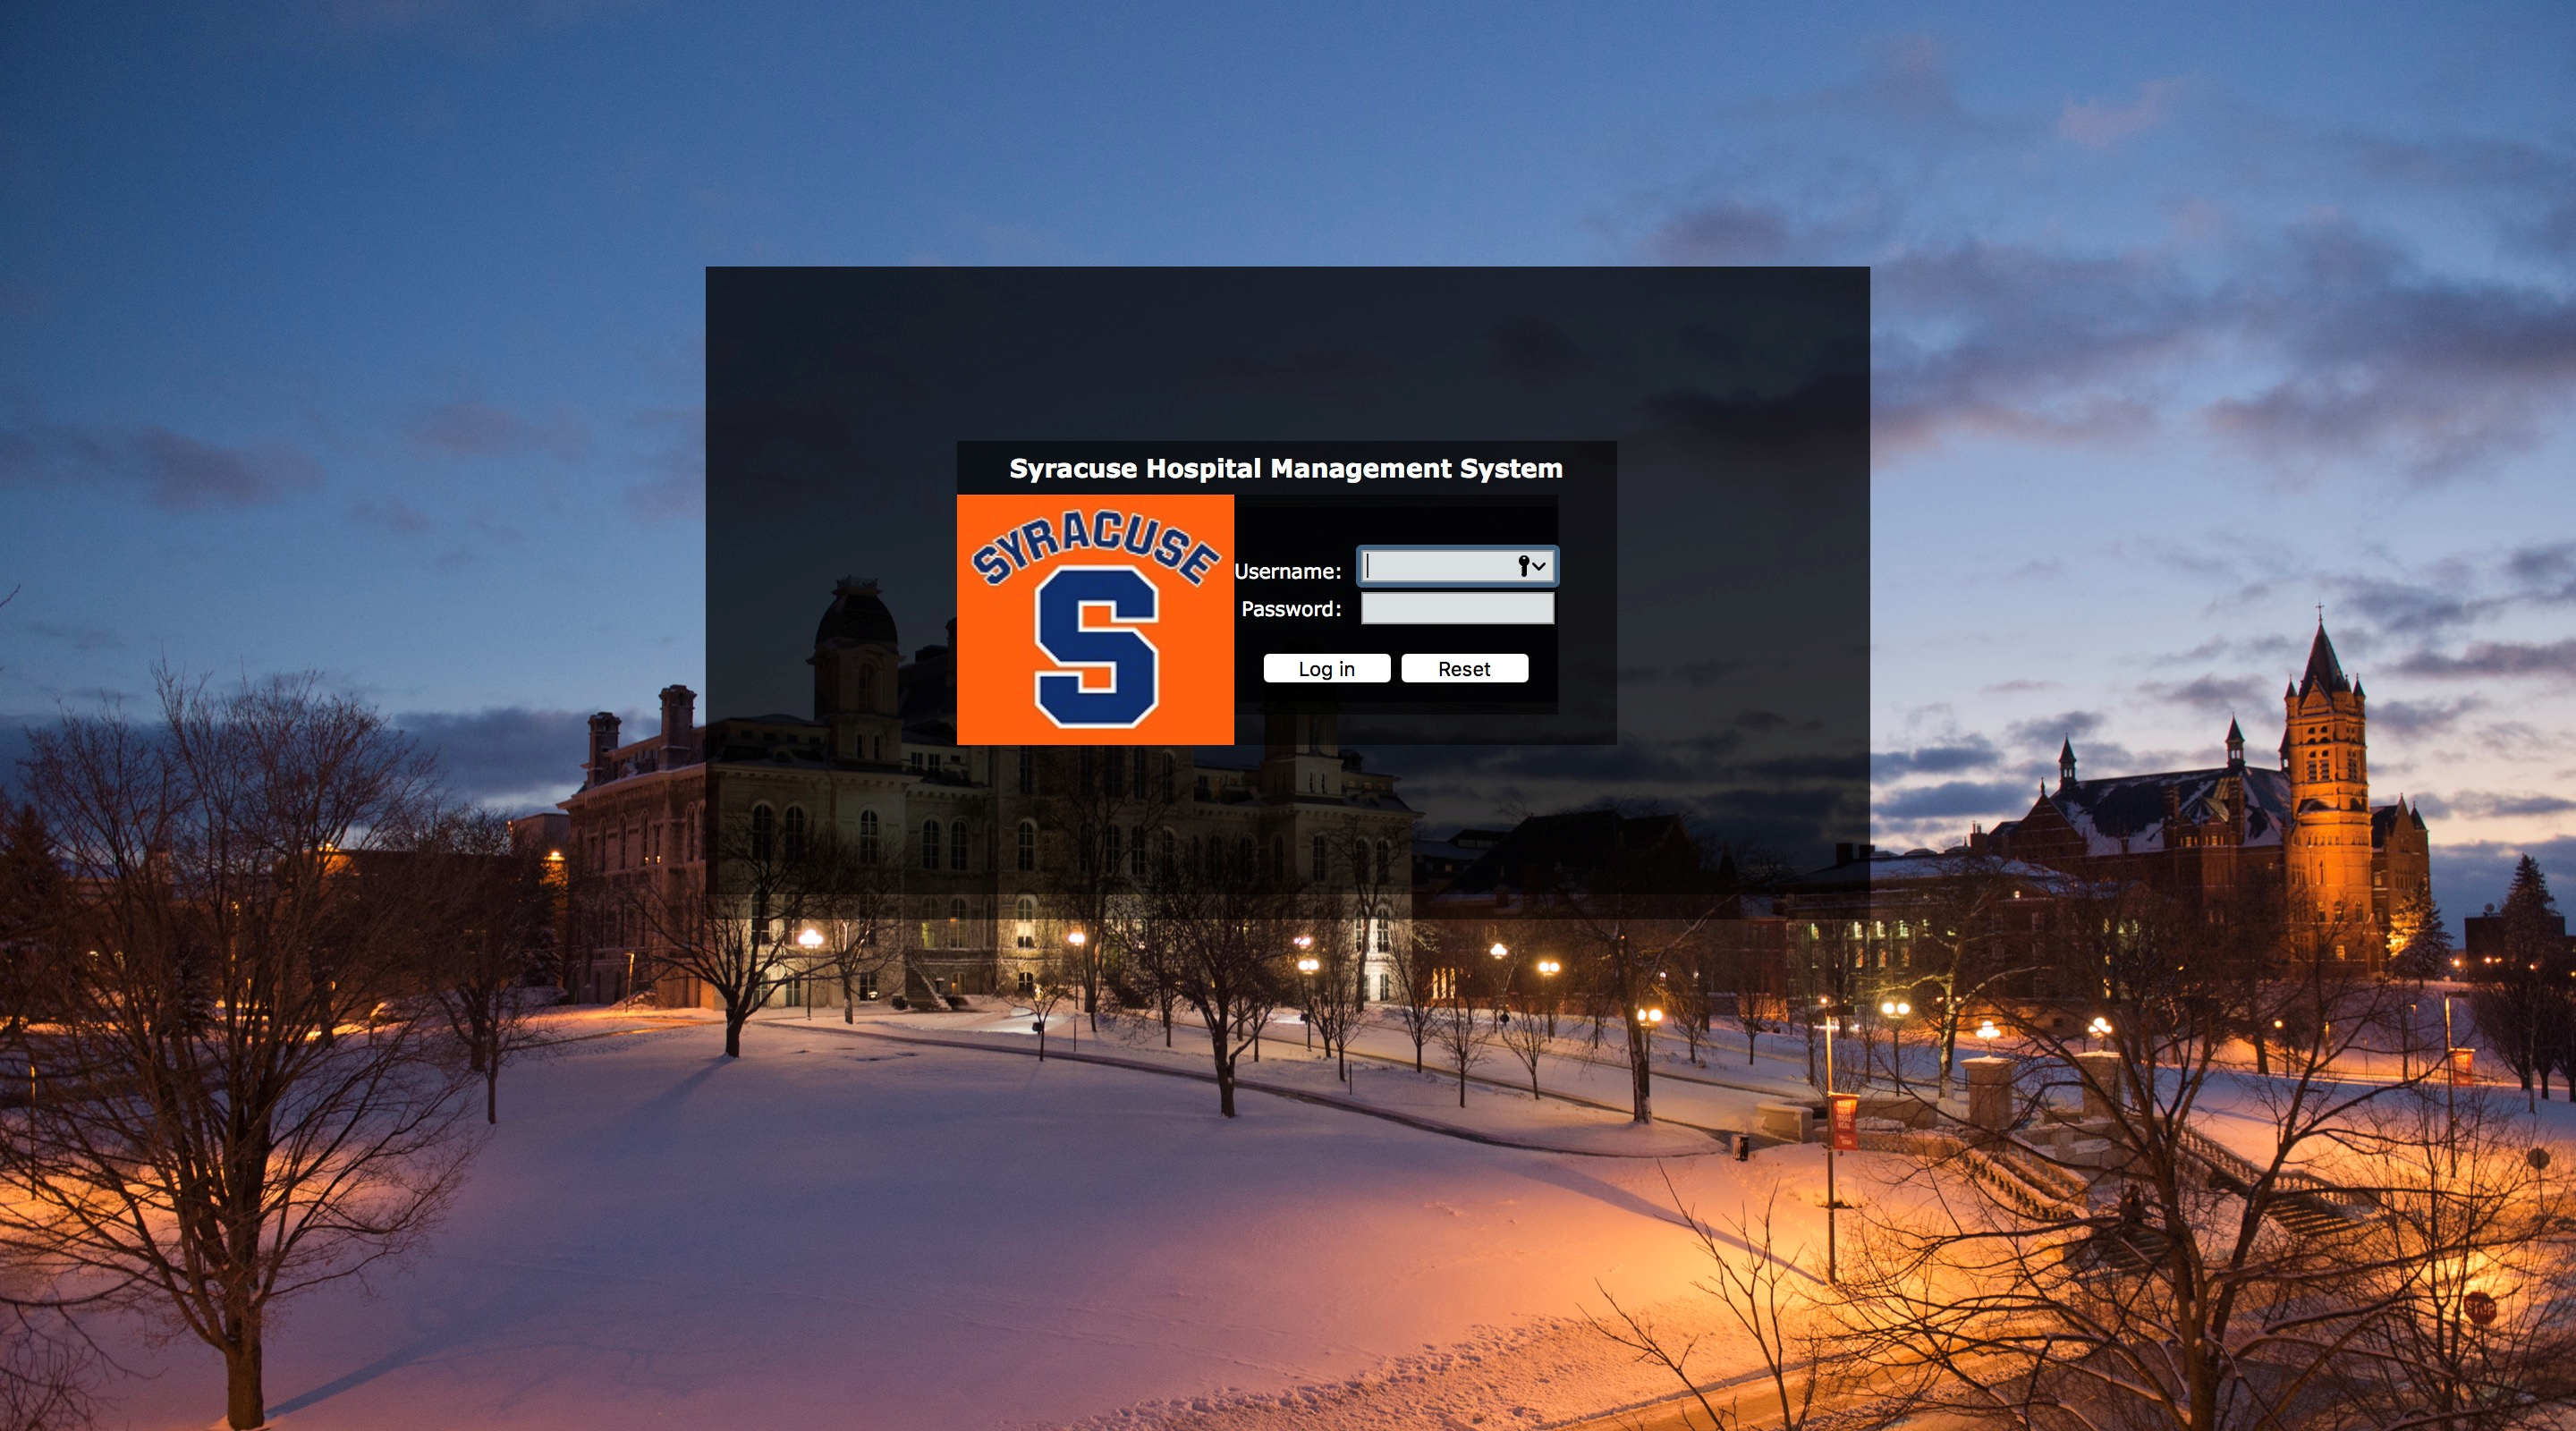
\includegraphics[width=\textwidth]{7.png}
    \caption{Interface}
    \label{fig:p7}
\end{figure}
Relative functions:

\begin{enumerate}
    \item As we can see, this interface consists of two input boxes and two buttons. After the user enters his own information into the corresponding input box, click the login button to submit the data in the input box. 
    \begin{itemize}
        \item If the user enters the correct information, the system will let the client jump to the main page. 
        \item If there is any inconsistency, the corresponding error message is given.
    \end{itemize}
    \item Input: user name and password.
    \item Relevant processing: 
        \begin{itemize}
            \item First, the validity of the user name and password is checked through the check of the foreground JS, mainly to prevent the user from entering illegal characters. 
            \item After the verification of the front desk JS, the system will pass the user submitted data the day after tomorrow, let the server to check whether the user name exists or the password is correct.
        \end{itemize}
    \item Output: 
    \begin{itemize}
        \item If the user login is successful, he enters the user's system home page, and displays the related menu interface and provides the corresponding role operation according to the user's related type utype.
        \item If the login is unsuccessful, an error information page is displayed.
    \end{itemize} 
\end{enumerate}
\subsection{The realization of the main interface}
\subsubsection{Administrator main interface}
\label{sec:admin}
The administrator's main interface is expressed in the form of a menu, as shown in figure \ref{fig:p8}.
\begin{figure}[H]
    \centering
    \includegraphics[width=\textwidth]{8.png}
    \caption{Administrator interface}
    \label{fig:p8}
\end{figure}
The main functions are as follows:
\begin{enumerate}
    \item Staff management: The management of other roles except the system administrator, including the addition, modification, and deletion of their passwords and other detailed information, can also be performed on the user based on the user name and name.
    \item  Administrator user information: In addition to managing general employee information, administrators can also manage administrator related information, such as adding administrators.
    \item Log Management: Administrators can view and search the log information in the system, including searching according to the operator, and searching according to the operation record number. In this system, the log information is used in related operations, the system automatically in the database The relevant log information is inserted, where the log information is mainly divided into two types, one is an ordinary login operation, and the other is a new modification operation of the medical record, and the log records the operator, operation time and other related information.
    \item Modify personal information: Administrators can make some modifications to their own details.
    \item Modify login password: According to the existing password administrator, you can update your own password.
\end{enumerate}
\subsubsection{Reception main interface}
The window staff main interface is represented by a menu, as shown in Figure \ref{fig:p9}.
\begin{figure}[H]
    \centering
    \includegraphics[width=\textwidth]{9.png}
    \caption{Reception interface}
    \label{fig:p9}
\end{figure}
The main functions are as follows:
\begin{enumerate}
    \item Patient Registration: After the patient arrives at the hospital, the patient is registered at the window. The window personnel will register the relevant information and inform the patient of the patient's medical record number. The patient can find the doctor in the relevant department with the patient's medical record number.
    \item Prescription markup: When the doctor fills out the medical record and opens the benefits, the patient comes to the window with a good case for the prescription price.
    \item Prescription payment: After the prescription price is completed, the patient will perform the payment operation and calculate different according to whether the patient has medical insurance.
    \item Prescription medicine: After the patient completes the doctor's fee payment operation, he can go to the window to take medicine. However, if the patient has not paid, the window person cannot find the patient's medicine information in the medicine picking list.
    \item Modify Personal Information: The window personnel can modify their own details after logging in to the system.
    \item Modify login password: After logging into the system, the window personnel can update their own password based on the existing password.
\end{enumerate}
\subsubsection{Doctor's main interface}
The doctor's main interface is represented by a menu, as shown in Figure \ref{fig:p10}.
\begin{figure}[H]
    \centering
    \includegraphics[width=\textwidth]{10.png}
    \caption{Doctor interface}
    \label{fig:p10}
\end{figure}
The main functions are as follows:
\begin{enumerate}
    \item The patient: The doctor can find the patient's medical record according to the patient's medical record number and fill in the relevant information of the medical record.
    \item medical records view: doctors can search for relevant medical records based on different information of patients, including patient's name, ID number, medical record number and other relevant information.
    \item Prescription management: After the doctor fills out the patient's medical records, he can prescribe drugs to the patient. In this interface, the doctor can add prescription information, view the prescription information and find relevant prescriptions based on the medical record number and drug name, modify and delete. Related prescription information.
    \item modify personal information: After the doctor logs on the system can modify their own detailed personal information.
    \item modify the login password: Like other users, doctors can also follow their own password to keep up with their own password.
\end{enumerate}

\subsubsection{Warehouse keeper home screen}
The drug administrator is represented by a menu, as shown in Figure \ref{fig:p11}.
\begin{figure}[H]
    \centering
    \includegraphics[width=\textwidth]{11.png}
    \caption{Warehouse keeper interface}
    \label{fig:p11}
\end{figure}
The main functions are as follows:
\begin{enumerate}
    \item Drug basic information management: After the warehouse administrator logs in the system, he can add new drugs or modify existing drug information through the form, and can also query the corresponding drugs based on the drug name and applicable symptoms.
    \item Management of drug storage information: The library management personnel can add information on the storage of drugs, including information on time of storage, batch number of storage, etc., and can modify the relevant information of storage, and can also check according to the drug name and storage time. Related storage information.
    \item Drug inventory: The warehouse personnel can view the inventory information of the drug, including the inbound quantity, current inventory, total purchase amount and total sales, and purchase the goods according to the current inventory and sales.
    \item  modify personal information: inventory personnel can modify their own details after logging in the system.
    \item modify the login password: inventory personnel can log in to the system can update their own password based on the existing password.
\end{enumerate}


\section{Security Analysis}
In the section, we would like to discuss the potential attacks for our system, and our practical countermeasures to eliminate these risks. 

\subsection{SQL Injection}
\subsubsection{Introduction}
SQL injection is a code injection technique, used to attack data-driven applications, in which nefarious SQL statements are inserted into an entry field for execution (e.g. to dump the database contents to the attacker). 
 
Usually, it attacks by inserting an SQL statement into a data field, where only a number or string is wanted, to change the condition in where clauses or others. As a result, it may bypass some conditions to visit some pages or to view some table entries which should not be accessed by the attacker. 

\subsubsection{Attack Simulation}
This is extremely dangerous for our hospital management system, because an attacker may easily login as whatever role he wants, i.e. administrator, reception, doctor or warehouse.  Consequently, all secrete data like health history records, employee personal information will be stolen, and the data in the database may be modified or deleted.
 
Here is an example of how an attacker login as administrator using SQL injection. We insert such information in the login page.
\begin{figure}[H]
    \centering
    \includegraphics[width=\textwidth]{sp/sp1.png}
    \caption{Login with malicious input}
    \label{fig:s1}
\end{figure}
 
Click \emph{login} and see what will happen.
\begin{figure}[H]
    \centering
    \includegraphics[width=\textwidth]{sp/sp2.png}
    \caption{Login success}
    \label{fig:s2}
\end{figure}

\subsubsection{Countermeasure}
A most common countermeasure of SQL injection is ‘prepared statement’. It means to create a query format with question signs. When a query request is sent to database, we replace the question signs in the format with actual data. Whatever we write will be treated as data, rather than  a part of the query conditions. Luckily, there is such method provided in JAVA, we just have to use provided class to achieve the countermeasure. Here is the code.
\begin{figure}[H]
    \centering
    \includegraphics[width=\textwidth]{sp/sp3.png}
    \caption{Prepared Statement}
    \label{fig:s3}
\end{figure}
 
After applying prepared statement method, let’s try to repeat the attack. Here is the result.
\begin{figure}[H]
    \centering
    \includegraphics[width=\textwidth]{sp/sp4.png}
    \caption{Can't login}
    \label{fig:s4}
\end{figure}
 
As we can see, the attacker is unable to login as administrator now! SQL injection attack is prevented.

\subsection{CSRF attack}
\subsubsection{Introduction}
Cross-site request forgery, is a type of malicious exploit of a website where unauthorized commands are transmitted from a valid user that the target web application trusts. There are many ways in which a malicious website can transmit such commands. With a little help of social engineering (such as sending a link via email or chat), the attacker can lead the victim to access the malicious website, which may contains specially-crafted image tags, hidden forms, and JavaScript XMLHttpRequests, to send the unauthorized commands.
\subsubsection{Attack Simulation}
With CSRF attack, an attacker may trick the victim into executing actions of the attacker's choosing, without the victim approval. If the victim is a normal user, a successful CSRF attack can force the user to perform state changing requests like transferring funds, changing their email address, and so forth. If the victim is an administrative account, CSRF can compromise the entire target web application.

In our case, we write a malicious website to mock the behaviour of the attacker. After the victim login to the system, the victim access the malicious page and click submit. 
\begin{figure}[H]
    \centering
    \includegraphics[width=\textwidth]{sp/sp5.png}
    \caption{malicious website mock}
    \label{fig:s5}
\end{figure}
As a result, the victim’s password has been modified.
\begin{figure}[H]
    \centering
    \includegraphics[width=\textwidth]{sp/sp6.png}
    \caption{Before CSRF attack}
    \label{fig:s6}
\end{figure}
\begin{figure}[H]
    \centering
    \includegraphics[width=\textwidth]{sp/sp7.png}
    \caption{modify password success}
    \label{fig:s7}
\end{figure}
\begin{figure}[H]
    \centering
    \includegraphics[width=\textwidth]{sp/sp8.png}
    \caption{After CSRF attack, the password has beem modified}
    \label{fig:s8}
\end{figure}
\subsubsection{Countermeasure}


A practical countermeasure against CSRF is to ensure the request has the same origin with the web application domain. The referrer header, which can enable the new web page to see where the request originated, is a ideal target to verify whether the origin of request matches the target origin or not.  Since the Referrer header can be only set by the browser, checking the Referrer header becomes a commonly used method of preventing CSRF. 

In our case, we implement the Referrer header checking like the following Figure \ref{fig:s9}:
\begin{figure}[H]
    \centering
    \includegraphics[width=\textwidth]{sp/sp9.png}
    \caption{CSRF countermeasure}
    \label{fig:s9}
\end{figure}
After enabling the countermeasure, we can observe the forged request from the malicious website has been blocked.
\begin{figure}[H]
    \centering
    \includegraphics[width=\textwidth]{sp/sp10.png}
    \caption{Unauthorized request has been blocked}
    \label{fig:s10}
\end{figure}
\subsection{XSS attack}
\subsubsection{Introduction}
Cross-Site Scripting (XSS) attacks are a type of injection, in which malicious scripts are injected into otherwise benign and trusted web sites. XSS attacks occur when an attacker uses a web application to send malicious code, generally in the form of a browser side script, to a different end user. Flaws that allow these attacks to succeed are quite widespread and occur anywhere a web application uses input from a user within the output it generates without validating or encoding it.

\subsubsection{Attack Simulation}
An attacker can use XSS to send a malicious script to an unsuspecting user. The end user’s browser has no way to know that the script should not be trusted and will execute the script. Because it thinks the script came from a trusted source, the malicious script can access any cookies, session tokens, or other sensitive information retained by the browser and used with that site. These scripts can even rewrite the content of the HTML page. 

Here is an example to show how a malicious script is inserted to our website. We modify the full name of an employee to be a script. 
\begin{figure}[H]
    \centering
    \includegraphics[width=\textwidth]{sp/sp11.png}
    \caption{Input with script}
    \label{fig:s11}
\end{figure}
 
Then we let the administrator login, and visit employee information page in to see what will happen.
\begin{figure}[H]
    \centering
    \includegraphics[width=\textwidth]{sp/sp12.png}
    \caption{Improper input has been submitted}
    \label{fig:s12}
\end{figure} 
As we can see in Figure \ref{fig:s13}, there is an alert box shown in the page. It means that administrator’s username and password information will be stolen by the attacker, if we change the content of the script. Therefore, our website is a potential victim of XSS attack
\begin{figure}[H]
    \centering
    \includegraphics[width=\textwidth]{sp/sp13.png}
    \caption{Alert box}
    \label{fig:s13}
\end{figure} 

\subsubsection{Countermeasure}
To prevent this attack what we have to do is to remove or replace these sensitive characters or words. For example, we can replace $<$ and $>$ with \lbrack{} and \rbrack{} . As a result, the original script won’t be executed, because the string will never be treated as a script again.
 
Figure \ref{fig:s14} is how we implement it.
\begin{figure}[H]
    \centering
    \includegraphics[width=\textwidth]{sp/sp14.png}
    \caption{XSS countermeasure: Filtering}
    \label{fig:s14}
\end{figure}
 
Now we repeat the attack and let the administrator visit employee information page again. As we can see, the sensitive characters are replaced, therefore XSS attack is prevented.
\begin{figure}[H]
    \centering
    \includegraphics[width=\textwidth]{sp/sp15.png}
    \caption{Filtering works}
    \label{fig:s15}
\end{figure}

\subsection{Password Protection}
The protect of password is a critical block of the whole system. To achieve this, we implement two measures in our system.

\subsubsection{Hidden Password}
To prevent user’s password being pecked by others, we made it hidden when login or update password.
\begin{figure}[H]
    \centering
    \includegraphics[width=\textwidth]{sp/sp01.PNG}
    \caption{Hidden Password}
    \label{fig:s01}
\end{figure}

\subsubsection{Hashed Password}
Instead of storing the plaintext of user password, the server only keep the hash value of the user password. With secure hash function, our system can provide the security promise that the attacker can not recover the user’s password even if the sensitive data in the server leaks. Thus the password our user is secured.

We have completed the password hash processing part in Java, however implementing hashed password involves several parts of system modules, including adding new account, modifying password and information, and log in part. As a result, there are still some work to be finished in the future.

\begin{figure}[H]
    \centering
    \includegraphics[width=\textwidth]{sp/sp02.jpg}
    \caption{Hashed Password}
    \label{fig:s02}
\end{figure}
\section{System Evaluation and Analysis}

\subsection{Test Case}
In this section, we will show how to use our website by showing the process of how a patient goes to see doctor in hospital, as an evaluation of the whole system. All roles except administrator will be involved in this process. Considering that we have already discussed administrator’s functionality in Section \ref{sec:admin}. We won’t talk about it again.
\begin{figure}[H]
    \centering
    \includegraphics[width=\textwidth]{pp/pp1.jpg}
    \caption{Process}
    \label{fig:pp1}
\end{figure}
\begin{enumerate}
    \item When a patient enters the hospital, he first talks to a reception at front desk. And the reception will visit \emph{patient making appointment} page and create a health history record.
    \begin{figure}[H]
    \centering
    \includegraphics[width=\textwidth]{pp/pp2.jpg}
    \caption{patient making appointment}
    \label{fig:pp2}
\end{figure}
    \item Then the patient will visit the doctor. After the record is created, it will automatically appear in doctor’s \emph{Edit health history} Page, and doctor can edit it.
    \begin{figure}[H]
    \centering
    \includegraphics[width=\textwidth]{pp/pp3.jpg}
    \caption{Edit health history}
    \label{fig:pp3}
\end{figure}
    \item After editing the history, doctor can still review it in \emph{View health history} page.
    \begin{figure}[H]
    \centering
    \includegraphics[width=\textwidth]{pp/pp4.jpg}
    \caption{View health history}
    \label{fig:pp4}
\end{figure}
    \item Then doctor will create a prescription for this health history. Mentioning that if doctor want to use multiple different kinds of medicines, he just have to add multiple times with certain quantities.
    \begin{figure}[H]
    \centering
    \includegraphics[width=\textwidth]{pp/pp5.jpg}
    \caption{Edit prescription}
    \label{fig:pp5}
\end{figure}
    \item Now the patient can go back to see the reception again. The reception will visit \emph{Prescription pricing}, \emph{Prescription charging} and \emph{Prescription taking} page one by one to help the patient to pay for and to fetch medicine. 
    \begin{figure}[H]
    \centering
    \includegraphics[width=\textwidth]{pp/pp6.jpg}
    \caption{Prescription pricing}
    \label{fig:pp6}
\end{figure}
    \begin{figure}[H]
    \centering
    \includegraphics[width=\textwidth]{pp/pp7.jpg}
    \caption{Prescription charging}
    \label{fig:pp7}
\end{figure}    \begin{figure}[H]
    \centering
    \includegraphics[width=\textwidth]{pp/pp8.jpg}
    \caption{Prescription taking}
    \label{fig:pp8}
\end{figure}
    \item We can check \emph{Medicine summary} page before and after process 1 to 5. And we will see that the \emph{current inventory} row is decreased after this process.
\begin{figure}[H]
    \centering
    \includegraphics[width=\textwidth]{pp/pp9.jpg}
    \caption{Medical Summary}
    \label{fig:pp9}
\end{figure}
\end{enumerate}

\subsection{Main functionality}
\subsubsection{Main functionality}

This project focus on the information processing problems in real-time hospital scenarios, including the whole process from appointment to prescription. And our main goal is to achieve rapid response and high efficiency in hospital information management situations. The system mainly includes user management, medical record management, prescription management, warehouse management, log management, etc.

\subsubsection{Details}
\begin{itemize}
    \item Based on the actual demand in hospital situation, we conclude the lightweight design of the hospital management system, which achieves low system requirements.
    \item we choose moderate open-source MySQL as our database management system and connect it with basic JDBC API, which provide with easy adoption and scalability support based on further demands.
    \item Roles defined in the system are clearly separated and the functionality of  modules can meet the requirements of hospital scenarios. Our UI design is concise, clear and user-friendly, thus users can easily find the information and finish their operations without additional guidance.
    \item Thanks to the strong capability and cross-platform functionality of Java, our system can be implemented on various platforms, and support multiple devices with little effort.
    \item We implement several security countermeasures to eliminate the risk of various potential attacks, including SQL injection attack, CSRF and XSS attack. Therefore our system provide sufficient protection on sensitive information and user credentials in terms of confidentiality and integrity.
\end{itemize}

\subsection{Features}
\subsubsection{Log Management}
Event logs record events taking place in the execution of a system in order to provide an audit trail that can be used to understand the activity of the system, to diagnose problems and to recover from incorrect actions. In our hospital management system, we keep record of all employee actions, such as login, creating prescription and medicine into warehouse.

With this log table, the website is much more maintainable for administrator
\begin{figure}[H]
    \centering
    \includegraphics[width=\textwidth]{fp/s1.png}
    \caption{Log Management}
    \label{fig:sp1}
\end{figure}
\subsubsection{Coherence and streamlined}
It is our goal to design a highly efficient and practical health center management website, which means that different roles don’t have to consider interaction with other roles and that our server will assist them to achieve interaction. Therefore, coherence is an import part of our design. There is coherence everywhere in our system.
\begin{figure}[H]
    \centering
    \includegraphics[width=\textwidth]{fp/s2.png}
    \caption{Coherence}
    \label{fig:sp2}
\end{figure}
\begin{enumerate}
    \item Reception and Doctor
    
    After a reception makes an appointment for a patient, a fresh unedited health  history record will automatically be created in doctors’s \emph{edit health history page}. After editing it, a doctor can create prescription for this history record. After that, a prescription will automatically appear in reception’s \emph{prescription pricing} page. 
    \begin{figure}[H]
    \centering
    \includegraphics[width=\textwidth]{fp/s3.png}
    \caption{Edit health history record}
    \label{fig:sp3}
\end{figure}
    \item Reception and Warehouse Keeper
    
    After a reception charges and takes medicine for a patient. This action is automatically record to our database, and the amount of available medicine in the warehouse is automatically decreased.
\end{enumerate}

\subsubsection{Detail oriented}
To make our website as real and practical as possible, we focus on detail as best as we can. 

\begin{itemize}
    \item We make updating password logic and all other actions atomic and rigorous. 
    \item We apply a lot of format constraints to simulate real personal information.
        \begin{figure}[H]
    \centering
    \includegraphics[width=\textwidth]{fp/s5.png}
    \caption{Constraint 1}
    \label{fig:sp5}
\end{figure}
\begin{figure}[H]
    \centering
    \includegraphics[width=\textwidth]{fp/s6.png}
    \caption{Constraint 2}
    \label{fig:sp6}
\end{figure}
\begin{figure}[H]
    \centering
    \includegraphics[width=\textwidth]{fp/s7.png}
    \caption{Constraint 3}
    \label{fig:sp7}
\end{figure}
\end{itemize}


\section{Conclusion and Future Plan}
\subsection{Conclusion}
After two months’ effort of all our 8 members, we successfully build this health center, with both front-end and back-end side developed by ourselves.  Our team mainly focus on how to make the website practical and secure.

To make the system practical, we put a lot of thoughts on how make a coherent and streamlined process and implementation details. For example, we did pattern validation, passed a fresh appointment to doctor’s page, etc. 

Considering that there are many sensitive information stored in hospital, we tried our best to make the website. We implemented a log table and managed to avoid many potential security problems. Consequently, the website is easy to maintain and difficult to attack.

Though we had thought of creating a role for patients, we decided not to include it after consideration. We designed this website for hospital internal use, and whatever patients want to do can be done with reception’s assistance. Moreover, adding a patient role may greatly increase the attack surface of our website.

\subsection{Future Plan}
\begin{enumerate}
    \item Complete password hashing. 
    
This is an important fail safe strategy. If only hash values of passwords of users are stored in our database, attackers will never know the actual passwords of users. We are about to finish it!
    \item Improve health history management
For now, all doctors can view all health history. We are planning to make doctors only able to view health histories related to him. The less privilege, the better! :)

\end{enumerate}

\newpage 
\section*{Thanks to Dr. Yu and TAs!}


\end{document}
